In this section, we examine our experimental results to address the research questions defined in the experiment.

\begin{figure}[t]
 \centering
  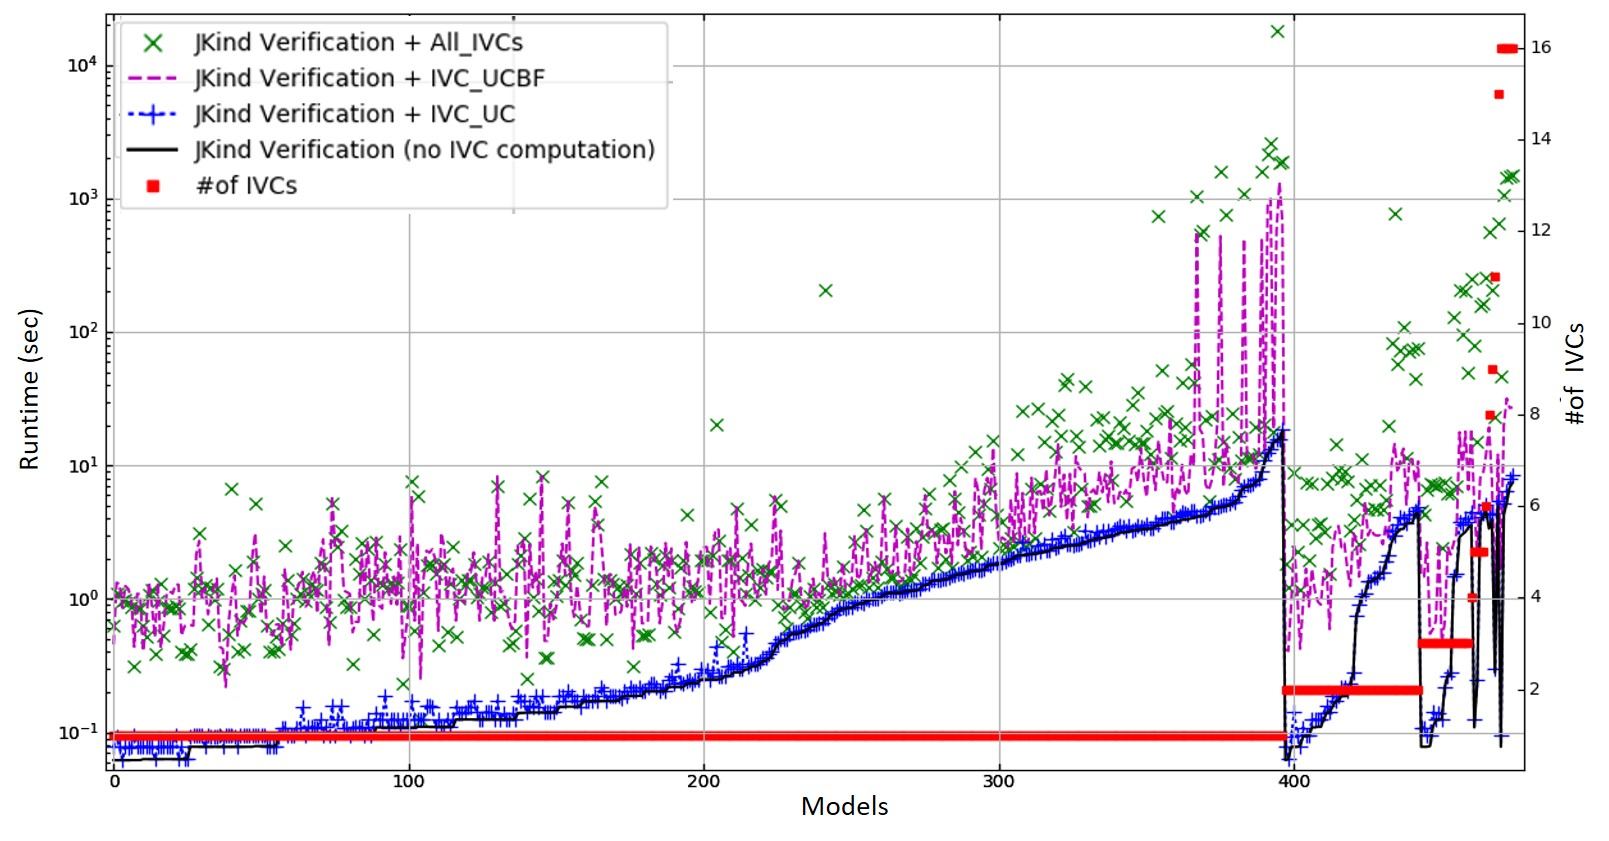
\includegraphics[width=\textwidth]{figs/performance.jpg}
  \label{fig:performance}
  \vspace{-0.2in}
  \caption{Runtime of \aivcalg, \ucbfalg, and \ucalg ~algorithms}
\end{figure}
%\vspace{0.1in}

\subsubsection{RQ1:} 

To address RQ1, we measured the performance overhead of the various IVC algorithms against the baseline time
necessary to find a proof using inductive model checking. Fig. \ref{fig:performance} provides an overview of the  overhead of the \aivcalg ~algorithm in comparison to the \ucalg ~and \ucbfalg\ algorithms.  In the figure, each curve is ranked along the x-axis according to the time required for the algorithm to terminate for each analysis problem.  Table \ref{tab:runtime} and Table \ref{tab:overhead} provide a summary of the computation time and the overhead of different algorithms, respectively.  As is evidenced by Fig. \ref{fig:performance}, the \ucalg\  algorithm imposes a negligible overhead over the baseline proof time, whereas both the \ucbfalg\ algorithm and \aivcalg\ algorithms add a substantial penalty over the baseline proof time.  We examine the performance of the \aivcalg\ algorithm both in terms of the time required to find all IVCs and also the time required divided by the number of IVCs found.  Somewhat surprisingly, for the majority of models, the latter measure outperforms the \ucbfalg\ algorithm for the majority of the models in the benchmark suite.

The \aivcalg\ algorithm requires approximately 3.4x more time than the \ucbfalg\ algorithm, calculated in the following way: we measure the ratio of time required for each model for both metrics, then we take the mean over all models of this ratio.  It is important to note that these performance curves are sensitive to the timeout values chosen for individual proof-searches for IVCs (the \getivc\ step in \aivcalg and line 3 in the ``brute force'' algorithm in~\cite{Ghass16}).  This will be discussed in more detail in Section~\ref{sec:experiment-discussion}.

%The \aivcalg ~algorithm could have had better (worse) performance
% if timeout had been set lower (higher), which caused the average runtime (overhead) of the \aivcalg ~shown in Table \ref{tab:runtime} (Table \ref{tab:overhead}) to be $\thicksim 3$ times more than \ucbfalg .


\begin{table}
  \caption{Runtime of different computations}
   \vspace{-0.1in}
  \centering
  \begin{tabular}{ |c||c|c|c|c| }
    \hline
      runtime (sec)& min & max & mean & stdev \\[0.5ex]
    \hline\hline
    \emph{\small{proof-time}}    & 0.047 & 14.617 & 1.299 & 1.940 \\[0.5ex]
    \aivcalg    & 10.125 & 2375.058& 58.884 & 256.529 \\[0.5ex]
    \ucbfalg &   0.248 & 1323.515 &  17.247& 104.838\\[0.5ex]
    \ucalg&  0.0  & 1.422  & 0.084 & 0.184 \\[0.5ex]
    \hline
  \end{tabular}
  \label{tab:runtime}
\end{table}

\begin{table}
  \caption{Overhead of different algorithms}
   \vspace{-0.1in}
  \centering
  \begin{tabular}{ |c||c|c|c|c| }
    \hline
     algorithm & min & max & mean & stdev \\[0.5ex]

    \hline
    \aivcalg   & 13.642\% & 101034.615\% & 2544.399\% & 7764.159\% \\[0.5ex]
    \ucbfalg &   14.092\% & 111124.432\% &  882.018\% & 1512.071\%\\[0.5ex]
    \ucalg&  0.00\%  & 100.00\%   & 10.226\% & 11.718\% \\[0.5ex]
    \hline
  \end{tabular}
  \label{tab:overhead}
\end{table}

%\takeaway{Computing all minimal Inductive Validity Cores with the \aivcalg ~algorithm is as nearly expensive as computing one single minimal Inductive Validity Core with the \ucbfalg  ~algorithm.
%\ela{Ela: is that fair to say??}}
\vspace{0.1in}
\subsubsection{RQ2:} For this research question, we examine how the proof time of the original model and the number of MIVCs associated with the property affects the analysis time of the \aivcalg\ algorithm.  Figure~\ref{fig:modelsize} provides an overview of this data.  The data in Figure~\ref{fig:modelsize} is sorted twice along the x-axis: the major axis is the number of IVCs that exist for the model, and the minor axis is the analysis time of the baseline model.  In this graph, we can visualize how both factors effect the performance of the \aivcalg\ algorithm.  Note that there are two scales for the y-axis: the scale on the left is a logarithmic scale of performance in terms of the run time; the scale on the right is a linear scale based on the number of minimal IVCs discovered.

Figure~\ref{fig:modelsize} shows two distinct trends.  First, for models whose baseline proofs are inexpensive and that only have a single MIVC, the \aivcalg\ is roughly equivalent in performance to the \ucbfalg.  However, as proofs become more expensive for a single MIVC, the \aivcalg\ begins to underperform the \ucbfalg.  This trend becomes more pronounced for properties that yield multiple MIVCs.  In the cases where several MIVCs are found, the \aivcalg\ algorithm can underperform the \ucbfalg\ algorithm by an order of magnitude.  Thus, the performance of the \aivcalg\ is driven to a large degree by the number of minimal inductive validity cores that exist for the model.


%The structure of the model and specification can play a part in how well \aivcalg ~performs.
%Therefore, we would like to examine whether or not there is a relationship between the performance and the size of the model, proof-time, and the diversity of IVCs. A graph showing the size of each model (determined by the number of equations in the model) and the number of IVCs
% along with the running time of \aivcalg ~and normal verification time is shown in Fig \ref{fig:modelsize}. In the figure, the models are ranked along the x-axis by their size. The picture shows that as models get larger, it is more likely for the \aivcalg ~algorithm to take more time to complete. However, there is no straightforward relationship between the performance and the number of IVCs. It can be expected that the running time of the \aivcalg ~algorithm goes higher when verification takes more time.

 \begin{figure}[t]
 \centering
  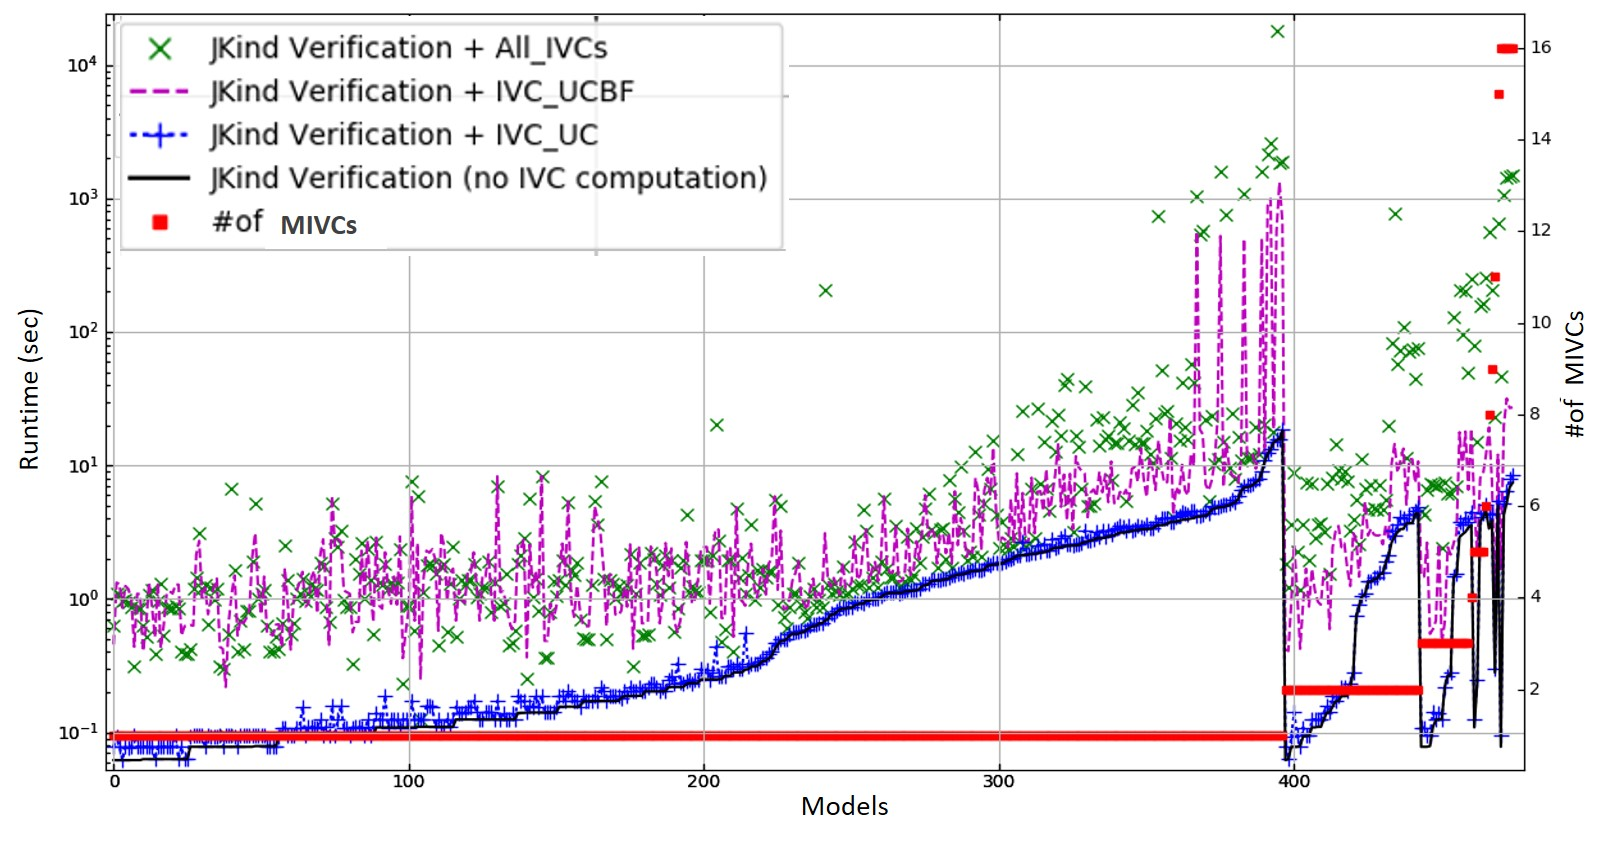
\includegraphics[width=\textwidth]{figs/size.jpg}
  \label{fig:modelsize}
  \vspace{-0.2in}
  \caption{Runtime of different computations along with the number of IVCs}
\end{figure}

%\ela{do we want this table 3? I commented the table description in case you want to use it...}
%Table \ref{tab:ivcsize} compares
%the  minimum,  maximum,  average,
%and standard deviation of the size of the IVCs computed by the different algorithms.
%For the \aivcalg ~algorithm, the  minimum,  maximum,  average,
%and standard deviation of the size of the IVCs per model is calculated, and then again, these four measures are calculated among all models.
%As for the \texttt{minimum IVC} row, the four measures are calculated among the size of the minimum IVC generated by \aivcalg ~for each model.
%The size of IVCs computed by \ucalg ~and \ucbfalg ~are quite close to each other. It means the \ucalg ~algorithm computes IVCs that are very close to the minimal ones obtained from the \ucbfalg , which makes the \ucalg ~algorithm a reasonable choice for the \getivc ~procedure in Algorithm \ref{alg:aivc}
%although it does not guarantee minimality.
%Fig. \ref{fig:ratio} also demonstrates that average cost of \aivcalg ~per IVC is very close to average cost of finding one IVC by \ucbfalg. Given the fact that the size of IVCs generated by \ucalg ~is very close to the ones generated by \ucbfalg, makes the \ucalg ~algorithm
%more efficient for the \getivc ~procedure.
\begin{table}
  \caption{Size of IVCs from different computations}
   \vspace{-0.1in}
  \centering
  \begin{tabular}{ |c||c|c|c|c| }
    \hline
     algorithm & min & max & mean & stdev \\[0.5ex]

    \hline
    \aivcalg   & 1 & 159 & 12.462 & 1.1684 \\[0.5ex]
    \ucalg   & 1 & 141 & 12.754 & 16.000 \\[0.5ex]
    \ucbfalg &   1 & 141 &  12.185 & 16.107\\[0.5ex]
    \texttt{minimum IVC} & 1  & 134  & 12.078 & 15.550 \\[0.5ex]
    \hline
    \end{tabular}
  \label{tab:ivcsize}
\end{table}

 %\begin{figure}
% \centering
%  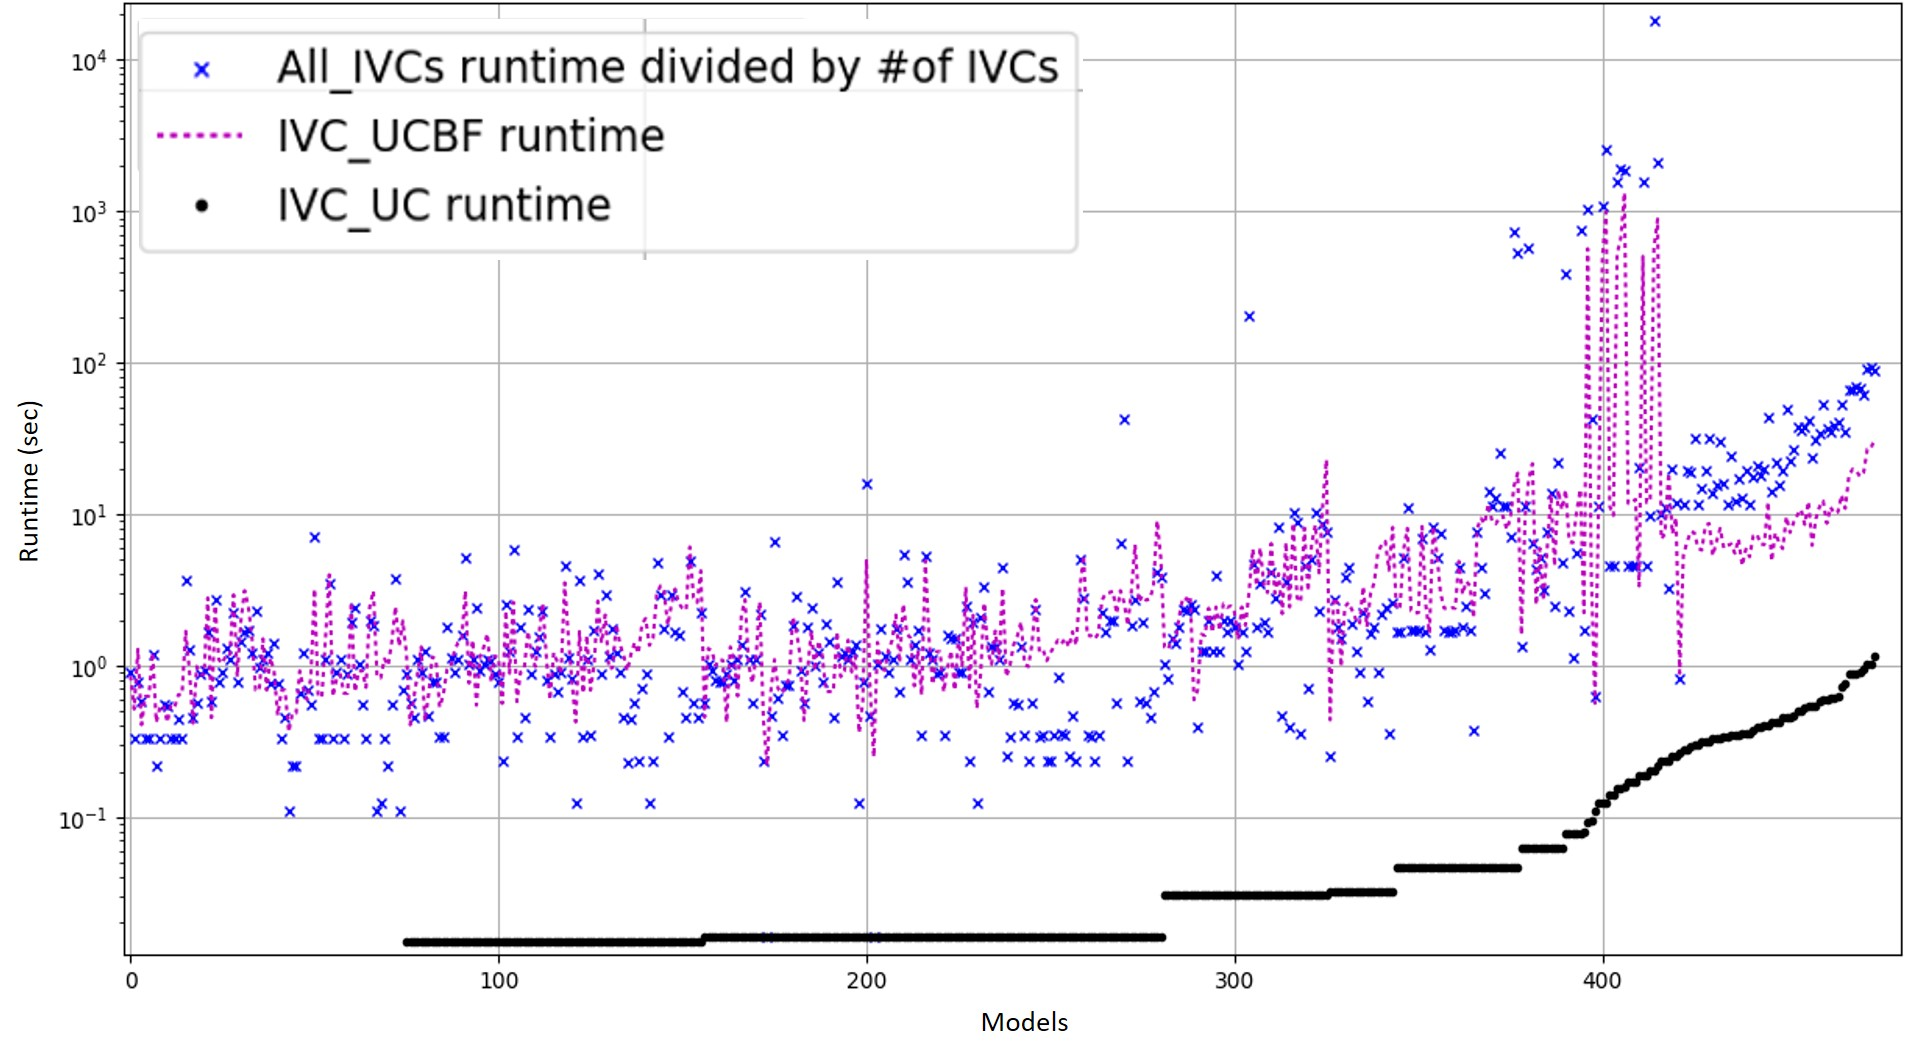
\includegraphics[width=\textwidth]{figs/ratio.jpg}
%  \label{fig:ratio}
%  \vspace{-0.2in}
%  \caption{Runtime of \aivcalg ~along divided by the number of IVCs vs the runtime of other computations}
%\end{figure}
\subsection {Discussion}
\label{sec:experiment-discussion}
\ela{rewrite...\\}
\textbf{RQ4)} In the benchmarks, there have been
several models containing undecidable cases which affected the average
performance of \aivcalg ~reported in Table \ref{tab:runtime}. Moreover, such cases also influence the minimality of the IVCs computed by \aivcalg. It is also possible that an iteration of
the \texttt{while} loop in Algorithm \ref{alg:aivc} times out while
the adequacy of the subset under examination is decidable in general.
We were interested in determining how often it is possible to come across such cases in our benchmarks. Size of IVCs obtained from different algorithms is shown in Fig. \ref{fig:min}.
As you can see, there are 14 cases among 476 models for which the size of
 minimum IVC computed by the \aivcalg ~is bigger than the size of the minimal IVC
 generated by the \ucbfalg ~algorithm.
 \begin{figure}
 \centering
  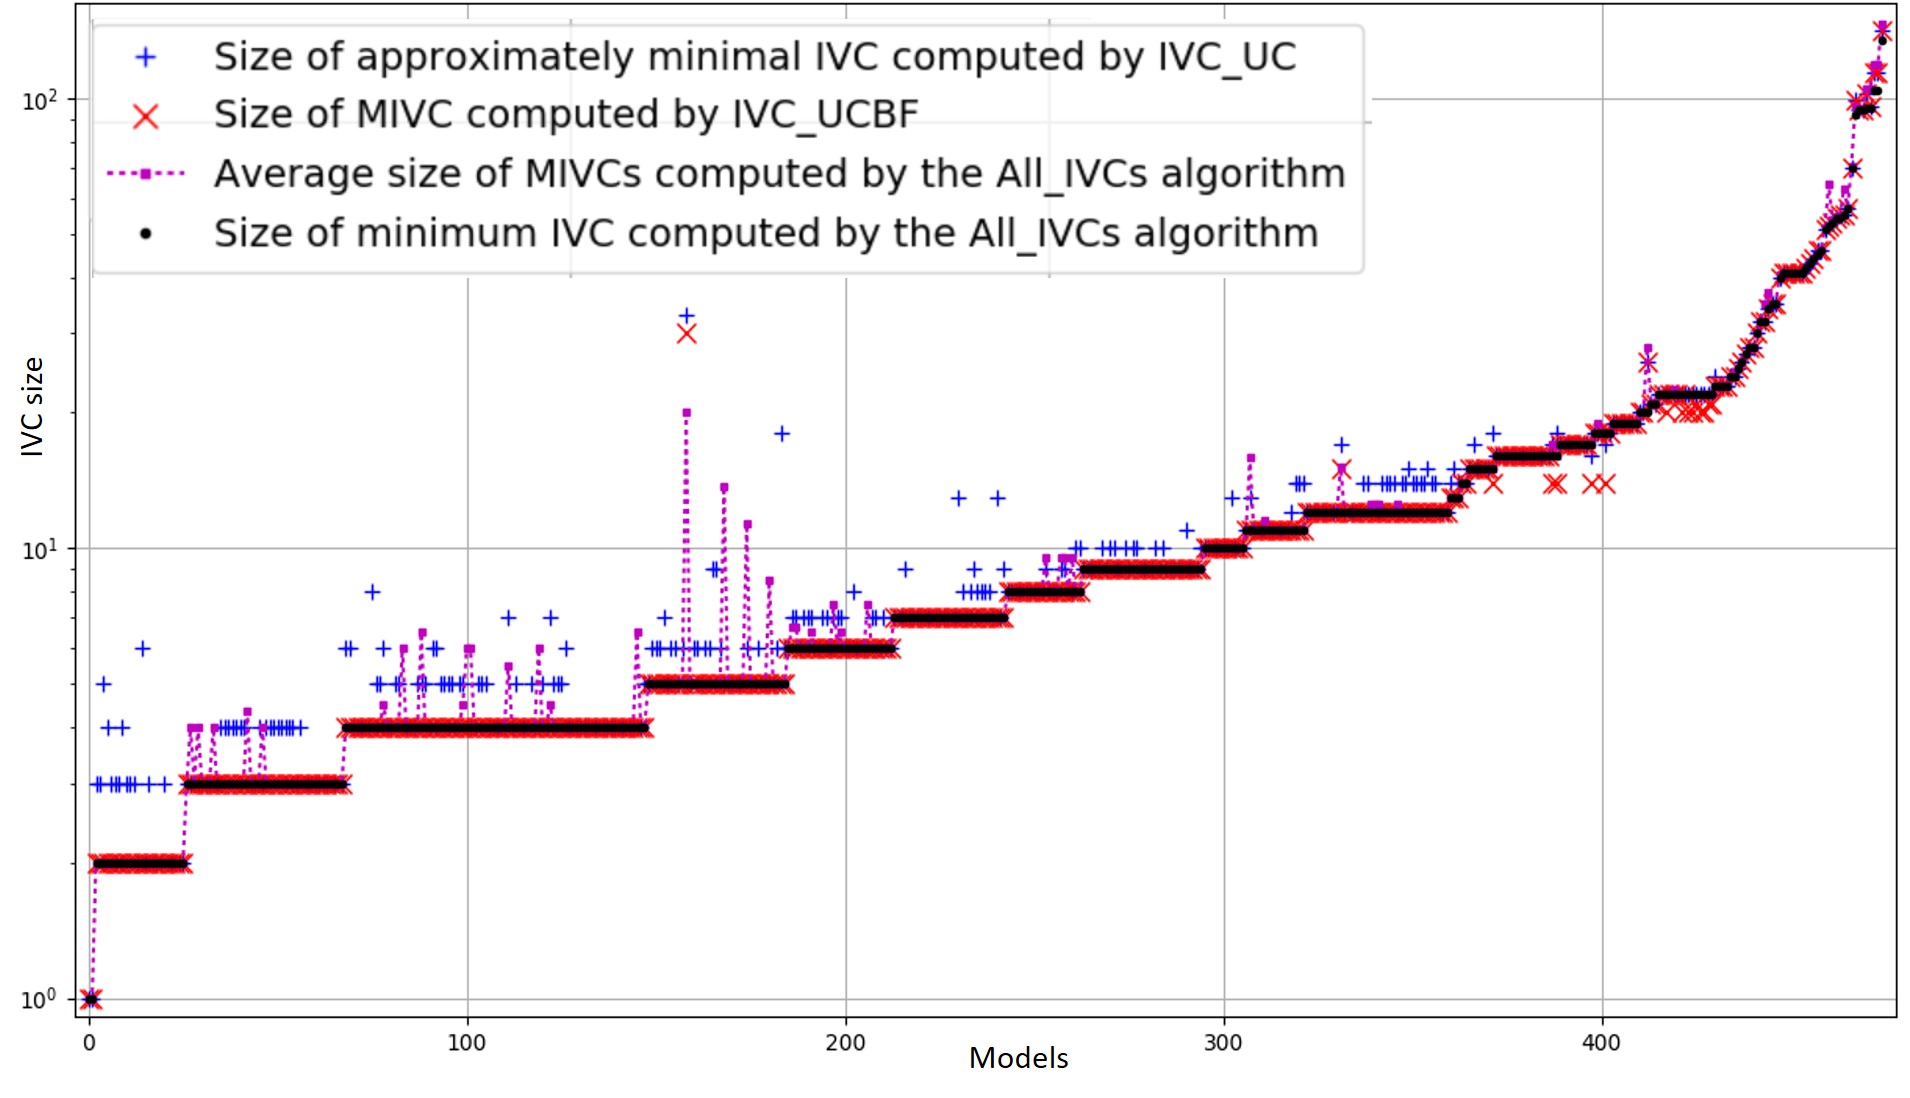
\includegraphics[width=\textwidth]{figs/min.jpg}
  \label{fig:min}
  \vspace{-0.2in}
  \caption{Size of IVCs obtained from different computations}
\end{figure}
